The sentiment dictionary is an essential element for large part of sentiment analysis approaches (\cite{Taboada:lexiconBased11, Rao:WWW14, Wen:AAAI14, Lee:IJCNLP2011}). The quality and the coverage of the sentiment dictionary affect the performance of sentiment analysis dramatically. However, it is not easy to obtain a sentiment dictionary with both high quality and wide coverage. For example, the well known ANEW \cite{Bradley:ANEW99} has hight quality sentiment values but only has 1,034 words. The situation is more rigorous in Chinese sentiment research. In previous work \cite{Strapparava:IREC04, Esuli:LREC06, Liu:IUI03, Cambria:AAAI10, Wu:TAAI11, Tsai:IEEE13, Wu:relSelect14}, researchers extend the existing sentiment dictionary by propagating the sentiment value of limit words on semantic networks like WordNet~\cite{Miller:WordNet95} or ConceptNet\cite{Havasi:RANLP07,Speer:LREC12}, successfully build larger lexicons at the cost of lower the quality. 

Many possible factors can cause the quality degradation in sentiment propagation, such as noisy data, sparse sentiment seeds \cite{Wu:relSelect14} and tricky network topology. We observed the propagation in previous approaches, and consider that not all types of links should be treat equally. For example, ``Desire'' and ``IsA'' are two types of links in ConceptNet, which have different meanings in real world. It doesn't make sense to assume they have the same power of conducting sentiments. In addition, we consider that not all neighbors should be treated equally. We usually mention the same concept in different topics, like there are both \textit{not go to work} in \textit{There is a Typhoon, we do not go to work today} and \textit{He is so ill and can not go to work today}, but two do not share the same sentiment value. Therefore, we argue that sentiment propagation should be topic dependent.

%Sentiment dictionaries tell machine how a writer or speaker may feel when using some term or phrase. They are important elements for several sentiment analysis approaches~\cite{Taboada:lexiconBased11, Rao:WWW14, Wen:AAAI14, Lee:IJCNLP2011}, but in Chinese, they are relatively scarce or non-public. As the result, it is helpful to collect the sentiment information in Chinese. However, there are two problems in collecting sentiment information. First, its coverage and quality highly affect the performance of sentiment analysis for texts, but collecting the information with high coverage, quality but low cost is challenging. The second problem is that the sentiments of several terms and phrases are context-dependent. How to define context, collect the sentiments on different contexts efficiently and decide which context and sentiment should be used to predict sentiments of texts are challenges.

%For the first problem, several approaches~\cite{Strapparava:IREC04, Esuli:LREC06, Liu:IUI03, Cambria:AAAI10, Wu:TAAI11, Tsai:IEEE13, Wu:relSelect14} have used the external knowledge such as WordNet~\cite{Miller:WordNet95} and ConceptNet~\cite{Havasi:RANLP07,Speer:LREC12} to build sentiment dictionaries automatically. The relationship information in WordNet and ConceptNet is used to propagate sentiments from some seeds, which had been compiled manually. 

%ConceptNet is a semantic network which represents knowledge into more computable representations. The nodes in ConceptNet are called {\it concepts} because the coverage of nodes contains not only lexical terms but also higher-order compound concepts, e.g., 'accomplish goal', 'leave behind'. A directed edge connecting two nodes is called {\it relation}, and is associated with one of the predefined types of labels to represent the semantic relationships between two {\it concepts} in real world, e.g., 'CapableOf', 'Causes'. The former {\it concept}, latter {\it concept} and their {\it relation} form an {\it assertion}, such as ``oven UsedFor cook", ``eat HasSubevent swallow". Because ConceptNet has large amount of {\it concepts} (In Chinese part~\cite{Kuo:HCOMP09,Kuo:FSS10}, there are at least 220000 {\it concepts}, still growing...), and its {\it concepts} have higher semantic meaning than traditional lexical terms, it is a good foundation to build a larger sentiment dictionary. In this paper, we collect sentiments based on {\it concepts} and the structure in Chinese ConceptNet.


% \begin{figure}[!t]
% \centering
% 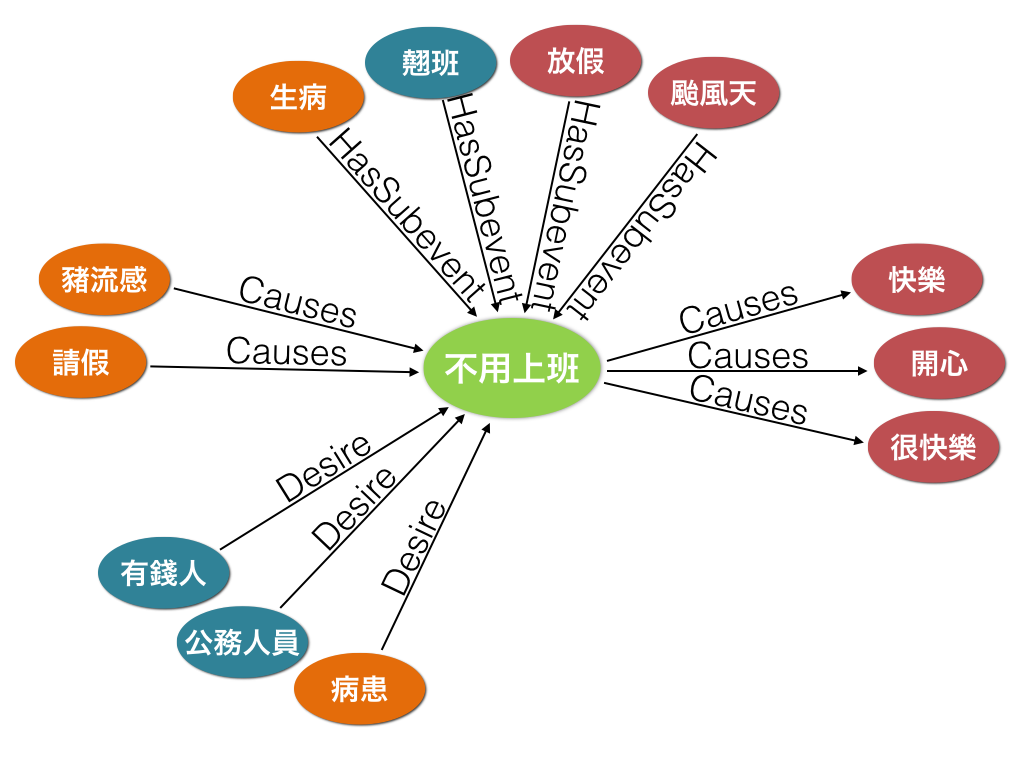
\includegraphics[width=3.2in]{fig/noWork2.png}
% \caption{Neighbors of 'do not have to work' come from different scenarios.}
% \label{fig:noWork2}
% \end{figure}

% The second problem is that each {\it concept} should be assigned different sentiments in different scenarios. For example, 'scream' is more possible to be negative when 'pervert' or 'cockroach' appears, but is more likely to be positive when 'idol' or 'win' appears. Previous approaches ~\cite{Xu:PACLIC10, Xu:COLING10, Rao:WWW14} use domain-specific corpus to modify sentiment value according to the corpus. However, hidden contextual information in Chinese ConceptNet is also abundant, like Figure~\ref{fig:noWork2}. If we could know which scenario an assertion belongs to, a {\it concept}'s sentiment in a scenario can be determined from its assertions which belongs to the scenario. 

In this work, we propose a topic-aware propagation approach to building sentiment lexicon based on Chinese ConceptNet. We extracted the hidden topics from the concept neighborhood with Latent Dirichlet Allocation~\cite{Blei:LDA03}. The sentiment propagation is performed on each latent topic separatly. Besides, we designed that each type of links has different impact on conducting sentiment values. The experiment results show that our approach outperforms than previous work. We also made a demo on how to apply this topic-aware sentiment dictionary to polarity analysis on the microblog dataset\footnote{\url{http://tcci.ccf.org.cn/conference/2013/pages/page04_dg.html}}.

The main contributions of this work are:
\begin{itemize}
  \item We propose the topic-aware propagation approach which can reduce the quality degradation in sentiment propagation.
  \item Our approach builds a topic-aware sentiment dictionary. With this dictionary, machine can make better sentiment prediction on text data.
\end{itemize}


